




% ######################################################################### %
% ------------------------------------------------------------------------- %
%                            Geometric Graphs
% ------------------------------------------------------------------------- %
% ######################################################################### %


\section{Geometric Graphs}\label{sec:geometric_graphs} 


The theory of geometric graphs addresses the embedding of graphs in
$\mathbb{R}^d$.  Planar graphs are graphs that can be drawn on a
surface with their edges drawn as straight lines between the vertices,
such that no two lines intersect
\parencite{Diestel_Graph-theory}. %Maybe West?
Here we are interested in graphs embedded on surface. In the models
introduced, connectivity then depends on geometric properties, such as
distance between nodes or relative orientation between vertices. The
basic graph type to allow for such connectivity rules is a geometric
graph.

\begin{definition}[Geometric directed graph]
  \index{geometric graph} 
  A \textit{geometric directed graph}
  $G_{\Phi}$ is a directed graph $G$ paired with a map
  \[
    \Phi:V(G) \to [0,1]^2,
  \]
  representing vertex positions on the unit square.
\end{definition}

This definition diverges from the usual notion of a geometric graph,
which determines the existence of edges only between nodes within a
spatial distance $x$ in a specified
norm \parencite{Penrose_Geometric-graph}. Moreover, geometric graphs
are usually only discussed in the context of random graph models, a
concept first introduced by \textcite{Gilbert1961}. Denote the set of
geometric graphs with $n$ edges by $G_{\Phi}^n$. The spatial embedding
of geometric graphs allows us to define (random) connectivity
depending on vertex positions and inter-vertex distances.  Central to
this study is the distance-dependent random graph model, in which
edges are added with probability $p(x)$ depending on the distance $x$
between vertex pairs:

\begin{definition}[Distance-dependent random graph model]
  \label{def:distance_dependent_graph}
  \index{distance-dependent!random graph model}
  Let $n \in \mathbb{N}$ and $C: [0,\sqrt{2}] \to [0,1]$ a
  continuous %?? C0 analytic? 
  map.  A \textit{distance-dependent geometric random graph model}
  $G_{\Phi}(n,C)$ is a random graph model over $G^n_{\Phi}$, generated
  by distributing uniformly at random the $n$ vertices on the unit
  square and adding an edge from $v$ to $w$ for each vertex pair $(v,w) \in
  {V(G_{\Phi})}^2 \setminus \Delta_{V(G_{\Phi})}$ with a
  probability $C(x)$, depending on the distance $x = \norm{\Phi(v) -
    \Phi(w)}$ between the vertices.
\end{definition}

We call the function $C$ the graph's \textit{distance-dependent
  connection probability profile}\index{distance-dependent!connection
  probability}\index{distance-dependent!connection profile}.
Note that the connection profile is \textit{not} a probability
density but gives a probability of connection between a vertex pair
at distance $x$. 
%------------------------------------------------
% \marginpar{profile $C$ and distance distribution determine
%   connectivity}
%------------------------------------------------
Clearly, connectivity statistics in the distance-dependent graph model
intrinsically depend on the choice of $C$. To develop a thorough
understanding of connectivity in the model however, mapping the
distribution of inter-vertex distances is equally important. Here we
calculate the distribution of the distance between two random points
in a square of side-length~$s$. Being able to identify distributions
of transformed random variables is integral to the calculation:

\begin{lemma} \label{lemma:transform_random_variable} 
  Let $X,Y$ be independent continuous random variables with values in
  $\mathbb{R}$, denote with $f_X$ and $f_Y$ their probability
  distribution functions.%
  \begin{enumerate}[label=(\arabic*),ref=(\arabic*), itemsep=-0.6cm]
    \item The distribution of the random variable $X+Y$ is given by
      the probability density function%
      \[%
        f_{X+Y}(x) = \int_{\mathbb{R}} f_X(z) f_Y(z-x)\, dz.  
      \]% 
    \item The distribution of the random variable $X^2$ is given by
      the probability density function
      \[
        f_{X^2}(x) = %
        \begin{cases} 
          \frac{1}{2\sqrt{x}}\left(f_X(\sqrt{x})+f_X(-\sqrt{x})\right)
           & x > 0 \\           0     & x \leq 0 \\
        \end{cases}
      \]
    \item Let $X$ only take positive values. Then the distribution of
      the random variable $\sqrt{X}$ is given by the probability
      density function
      \[
        f_{\sqrt{X}}(x) = %
        \begin{cases}
          2x f_X(x^2) & x \geq 0 \\0   & x < 0 \\
        \end{cases}
      \]
  \end{enumerate}
\end{lemma}
%
% \begin{proof}
% Hello Proof
% \end{proof}

\begin{theorem} \label{theorem:distance_square}
  Let $D$ be a random variable mapping to the distance of
  two random points in the square $[0,s]^2$ of side-length $s$. Then the
  distribution of $D$ is given by the probability density function
  \vspace{0.25cm}
  \begin{align}\label{eq:distance_square}
    f(x) = \begin{cases} \frac{2 x^4 - 8 s x^3 + 2 \pi s^2 x}{s^4} & x \in
      [0,s]\\ \frac{H(x)}{s^4} & x \in [s,s\sqrt{2}),\\0 & x \notin [0,s\sqrt{2})
               \end{cases}
  \end{align}
  where
  \[
    H(x)=8 s x \sqrt{x^2-s^2} - 2x^3  
          - 4 s^2 x \left(1+\arcsin\left(1-\frac{2 s^2}{x^2}\right)\right).
  \]
\end{theorem}
%
\begin{proof}
  We follow the approach described by \textcite{Moltchanov2012}.
  Consider two independently and uniformly distributed random points
  $p_1 = (x_1,y_1)$ and $p_2 = (x_2,y_2)$ in $[0,s]^2$. The distance
  between $p_1$ and $p_2$ is given as
  \[
    \norm{p_1 - p_2} = \sqrt{(x_1 - x_2)^2 + (y_1 - y_2)^2}.
  \]
  As a first step we calculate the distribution for $\Delta_x = x_1 -
  x_2$. 
  % ------------------------------------------------
  % \marginpar{distribution for $\Delta_x = x_1 -  x_2$} 
  % ------------------------------------------------
  Denote with $f_{\Delta_x}$ its probability density. Then, since
  $f_{-x_2}(z) = f_{x_2}(-z)$,
  \begin{align}\label{eq:f_delta_x}
    f_{\Delta_x}(d) = f_{x_1 + (-x_2)}(d) = \int_{\mathbb{R}}  f_{x_1}(z)
    f_{x_2}(z-d)\, dz
  \end{align}
  after Lemma~\ref{lemma:transform_random_variable}.  % Klenke 14.19
  Density functions for $x_1$ and $x_2$ are given by
  \[
    f_{x_1}(z) = f_{x_2}(z) = %
    \begin{cases} 
      \frac{1}{s} & \mathrm{for} \, z \in  [0,s] \\
      0           & \mathrm{otherwise}.
    \end{cases}
  \] 
  Thus we may only obtain non-zero values in (\ref{eq:f_delta_x}) for $d
  \in (-s,s]$, as otherwise either one of the factors in the integrand
  is zero. In full we obtain the triangular distribution \parencite{Simpson1755},
  \begin{align*}
    f_{\Delta_x}(d) =  \begin{cases}
                         0 & d \notin (-s,s] \\
                         \frac{s+d}{s^2} & d \in (-s,0] \\
                         \frac{s-d}{s^2} & d \in (0,s].\\
                       \end{cases}
  \end{align*}  
  %
  Next we calculate the distribution for $\Delta_x^2 =
  (x_1-x_2)^2$. Using Lemma~\ref{lemma:transform_random_variable} once
  again we obtain for $d>0$
  \begin{align*}
    f_{\Delta_x^2}(d) & = \frac{1}{2\sqrt{d}}
    \left(f_{\Delta_x}(\sqrt{d}) + f_{\Delta_x}(-\sqrt{d})\right) \\
    & = \frac{1}{2\sqrt{d}} \left(\frac{s-\sqrt{d}}{s^2} +
      \frac{s+\left(-\sqrt{d}\right)}{s^2}\right) = \frac{1}{s\sqrt{d}} - \frac{1}{s^2},
  \end{align*}
  and $f_{\Delta_x^2}(d) = 0$ for $d \leq 0$. Note that of course,
  $f_{\Delta_x^2} = f_{\Delta_y^2}$ and we will refer to this density
  function as $f_\Delta^2$. Convolution yields again the probability
  density function for the sum of the random variables $\Delta_x^2$
  and $\Delta_y^2$,
  \begin{align*}%\label{eq:f_DeltaSum}
    f_{\Delta_x^2 + \Delta_y^2}(d) = \int_{\mathbb{R}} f_{\Delta^2}(z)
    f_{\Delta^2}(d-z)\, dz.
  \end{align*}

  Finally Lemma~\ref{lemma:transform_random_variable} lets us compute
  \begin{align*}%\label{eq:f_D}
  f_D(d) = f_{\sqrt{\Delta_x^2 + \Delta_y^2}}(d) = 2d\, f_{\Delta_x^2 +
    \Delta_y^2}(d^2),
  \end{align*}
  for $d \geq 0$, yielding expression (\ref{eq:distance_square}) for
   probability density function of $D$
   (Mathematica~\ref{mathematica:distances}, \ref{mathematica:comparison}). 
  % Otherwise, of course, $f_D(d) = 0$. Computing the
  % last two steps
  % % steps  (\ref{eq:f_DeltaSum}) and (\ref{eq:f_D}) 
  % in  Mathematica (see \autoref{mathematica:distances})
  % yields then expression (\ref{eq:distance_square}) for
  % probability density function of $D$. 
\end{proof}

The distribution for the distance between two random points in the
unit square $[0,1]^2$, is then obtained from
(\ref{eq:distance_square}) by setting $s=1$. The probability
density function $f$ becomes
  \begin{align}\label{eq:distance_unit_square}
    f(x) = %
      \begin{cases} 
        2 x^3 - 8 x^2 +  2 \pi x 
          & x \in [0,1) \vspace{0.15cm}\\ 
        8x \sqrt{x^2-1}-2x^3\\ 
        -4x- 4x\arcsin\left(1-\frac{2}{x^2}\right) 
          & x \in [1,\sqrt{2})
           \end{cases}
  \end{align}
  %
  % \begin{align}\label{eq:dist_pdf}
  %   f(x) = \begin{cases} 2 \pi x - 8 x^2 + 2 x^3 & x \in
  %     [0,s)\\ \begin{aligned} &8 x \sqrt{-1+x^2}-4 x-2 x^3\\ &-4 x
  %     \left(\frac{1}{\sqrt{-1+x^2}}\right)+4 x
  %     \arctan\left(\frac{1}{\sqrt{-1+x^2}}\right) \end{aligned}& x \in (1,\sqrt{2})
  %          \end{cases}
  % \end{align}
  % 
 
Plotting $f$ in combination with the results of a numerical simulation
($10000$ points randomly distributed on unit square, extracted
distances binned to a of width $\sqrt{2}/15$) verifies our calculation: 
%
%------------------------------------------------
\marginpar{\vspace{1.8cm}\\ label:
  \smtcite{01a179d9}\\ \smallskip More about labels
  in Appendix~\ref{sec:reproducibility}} 
%------------------------------------------------
\begin{figure}[H]
  \centering
  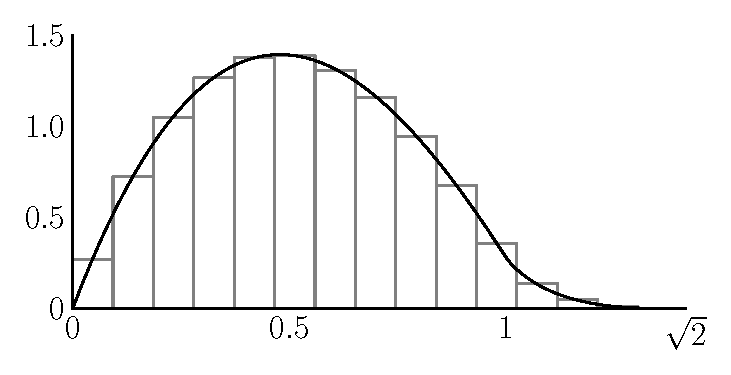
\includegraphics[width=0.7\textwidth, keepaspectratio]{%
    plots/01a179d9.pdf}%
  \label{fig:distance_distribution}
\end{figure}
%
\vspace{-0.8cm} Density functions \ref{eq:distance_square} and
\ref{eq:distance_unit_square} are of high importance. %?? Where when
Here we use \ref{eq:distance_unit_square} to compute the probability
that a random pair of vertices in the distance-dependent random graph
model is connected:

\begin{corollary}\label{th:distance_p} Let $v \neq w$ be vertices in an arbitrary
  realization of $G_{\Phi}(n,C)$. The probability $p$ for an edge
  from $v$ to $w$ is given by 
  \[
    p = \int_0^{\sqrt{2}} C(x) f(x) \, dx,
  \]
  where $f(x)$ is the probability density function~(\ref{eq:distance_unit_square}).
\end{corollary}

\textbf{Example} Let $C(x) = 1 - \frac{x}{\sqrt{2}}$. Then we compute
the probability to find an edge between a random vertex pair in
$G_{\Phi}(n,C)$ according to Theorem~\ref{th:distance_p} as
\[
  p = \int_{0}^{\sqrt{2}} f(x) \, dx - \frac{1}{\sqrt{2}}
  \int_0^{\sqrt{2}} x f_D(x) \, dx = 1 - \frac{1}{\sqrt{2}}\, \mathbf{E}[D].
\]
The expected distance between two random points on the unit square is
computed as $\mathbf{E}[D] \approx 0.521405$ (\autoref{mathematica:distances}),
a result confirmed by \textcite{Philip2007}. Thus we obtain the
probability for connection of $p \approx 0.631311$


%%% Local Variables: 
%%% mode: latex
%%% TeX-master: "../dplths_document"
%%% End: 
